%%%%%%%%%%%%%%%%%%%%%%%%%%%%%%%%%%%%%%%%%%%%%%%%%%%%%%%%%%%%%%%%%%%%%%%%%%%%%%%%
\chapter{Исследовательская часть}
%%%%%%%%%%%%%%%%%%%%%%%%%%%%%%%%%%%%%%%%%%%%%%%%%%%%%%%%%%%%%%%%%%%%%%%%%%%%%%%%

%%%%%%%%%%%%%%%%%%%%%%%%%%%%%%%%%%%%%%%%%%%%%%%%%%%%%%%%%%%%%%%%%%%%%%%%%%%%%%%%
\section{Описание контрольного примера}

Составим программу, которая будет менять скорость робота, основываясь на данных, полученных от датчика расстояния. Алгоритм такой программы приведен на рис. \ref{fig:program}.

\begin{figure}[htbp]
	\centering
	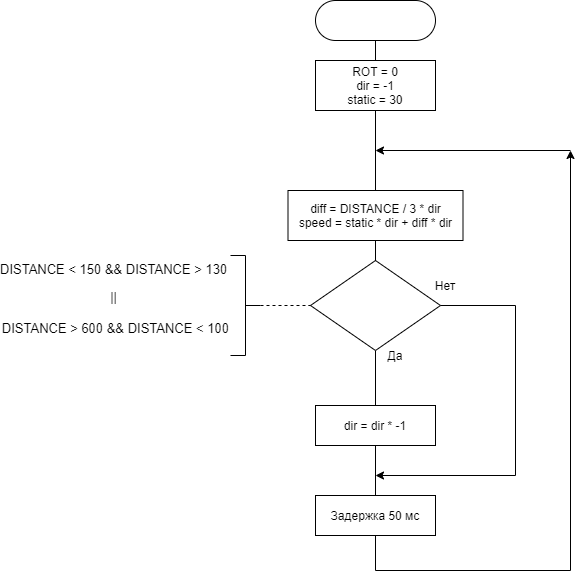
\includegraphics[width=\textwidth]{program.png}
	\caption{Алгоритм пользовательской программы}%
	\label{fig:program}
\end{figure}

Ее внутреннее представление в формате JSON имеет вид, приведенный в листинге \ref{listings:blocks}.

\nomenclature[2]{JSON}{JavaScript Object Notation}

\lstinputlisting[
label={listings:blocks},
caption={Внутреннее представление пользовательской программы},
style=javascript,
]
{listings/blocks.js}

После компиляции получаем массив команд и пользовательских переменных, приведенных в листингах \ref{listings:result-vars} и \ref{listings:result-inst}.

\lstinputlisting[
label={listings:result-vars},
caption={Внутреннее представление пользовательской программы},
style=javascript,
]
{listings/result-vars.js}

\lstinputlisting[
label={listings:result-inst},
caption={Внутреннее представление пользовательской программы},
style=javascript,
]
{listings/result-inst.js}

При запуске симуляции можно наблюдать, как меняется скорость робота в зависимости от расстояния до препятствия, что продемонстрировано на рис. \ref{fig:ui-run-1} и рис. \ref{fig:ui-run-2}.

\begin{figure}[htbp]
	\centering
	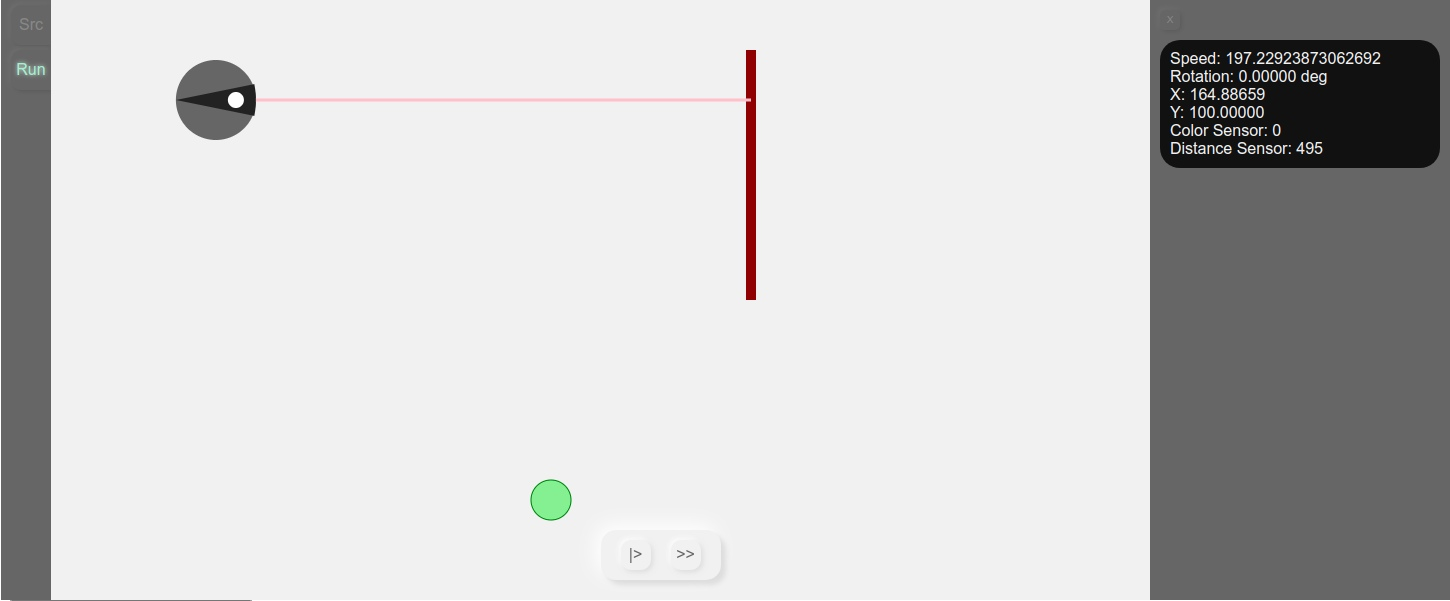
\includegraphics[width=\textwidth]{ui-run-1.jpg}
	\caption{Движение вдали от препятствия}%
	\label{fig:ui-run-1}
\end{figure}

\begin{figure}[htbp]
	\centering
	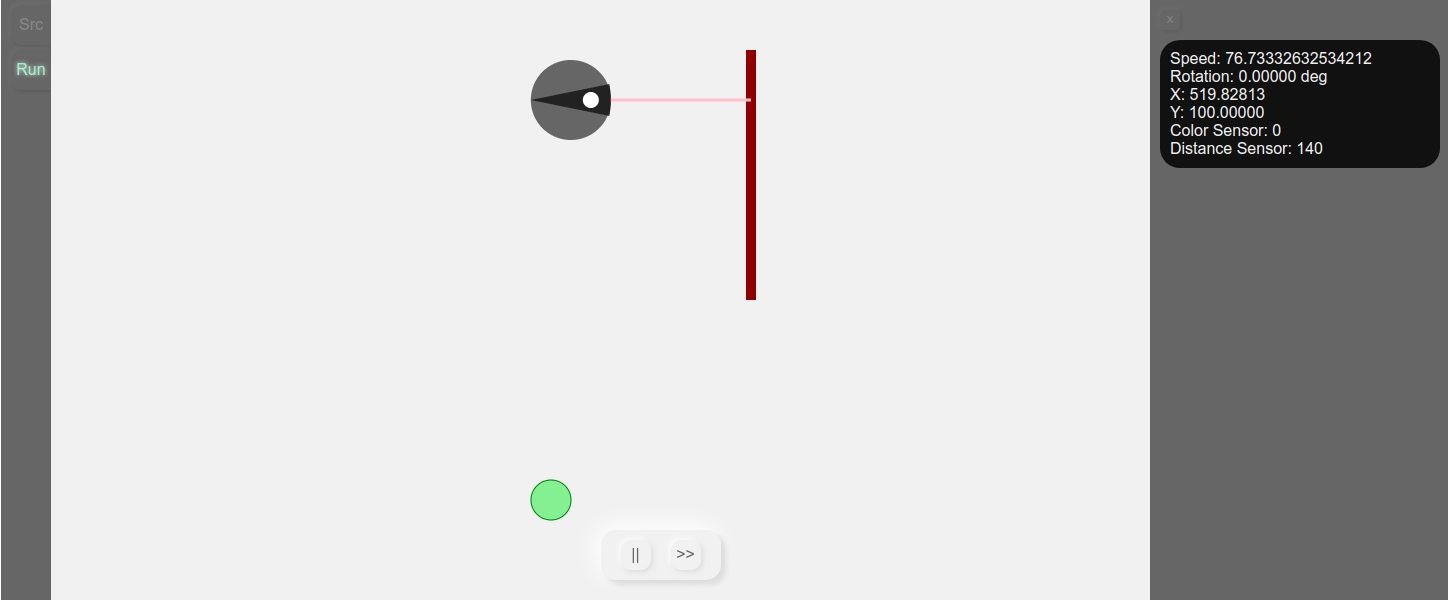
\includegraphics[width=\textwidth]{ui-run-2.jpg}
	\caption{Движение вблизи препятствия}%
	\label{fig:ui-run-2}
\end{figure}

Замеры времени выполнения одного цикла симуляции показывают, что время выполнения не превышает 1.5 миллисекунды, а в среднем составляет пример 0.02 миллисекунды, что является удовлетворительным результатом с учетом ограничения в 16.67 миллисекунд на один цикл. 

Технические характеристики устройства, на котором проводились испытания:

\begin{itemize*}
	\item Intel(R) Core(TM) i7-6820HQ CPU @ 2.70GHz;
	\item 16 GB DDR4 RAM;
	\item Intel UHD Graphics 620.
\end{itemize*}

\section{Дальнейшая разработка}

Как было описано выше, существуют возможности для расширения функциональности написанных модулей. Можно следующие ключевые направления дальнейшей разработки:

\begin{itemize*}
	\item расширение функциональности пользовательского интерфейса;
	\item увеличение количества переменных состояния робота и окружающей среды;
	\item расширение синтаксиса языка.
\end{itemize*}

В первом случае речь идет об улучшении пользовательского опыта в области редактирования программы для робота, выводе ошибок и т.п. Во втором - о добавлении дополнительных датчиков, а также о более гибкой их настройке (например, изменение угла наклона).

Наконец, расширение синтаксиса языка можно проиллюстрировать введением тригонометрических функций.

Кроме того, основные модули компонента написаны на чистом javascript, что делает возможным, при необходимости, их перенос с XBlock на любую другую технологию.

%%%%%%%%%%%%%%%%%%%%%%%%%%%%%%%%%%%%%%%%%%%%%%%%%%%%%%%%%%%%%%%%%%%%%%%%%%%%%%%%
